\documentclass[11pt]{article}
\usepackage[a4paper, left=0.75in, right=0.75in, top=0.5in, bottom=0.5in]{geometry}
\usepackage{amsmath, bm}
\usepackage{amssymb}
\usepackage{hyperref}
\hypersetup{
    colorlinks=true,
    linkcolor=blue,
    filecolor=magenta,      
    urlcolor=blue,
}
\usepackage{graphicx}
\graphicspath{ {.} }

\title{MSE 402 - Assignment 1}
\date{}
\author{Nishant Tatar - 21110223}

\begin{document}
\maketitle

\section{Question 1}
The Atoms are generated randomly inside the given constraints. Atoms or molecules overlapping over each other may occur due to random generation of positions. Overlap in positions results in a higher energy than what the system would have if all atoms were at the distance for minimal energy potential. Overlap is also physically impossible. Minimising the energy of a system takes care of overlapping atoms or molecules.\\ \\
While timestep is required in the lammps script for running the minimisation, this is because of calculation iterations. There is no time associated with energy minimisation, and the timestep provided in the script is the number of iterations to calculate for. Energy Optimisation is Positional.

\section{Question 2}

\textbf{2} water molecules crossed through membrane 1. \\
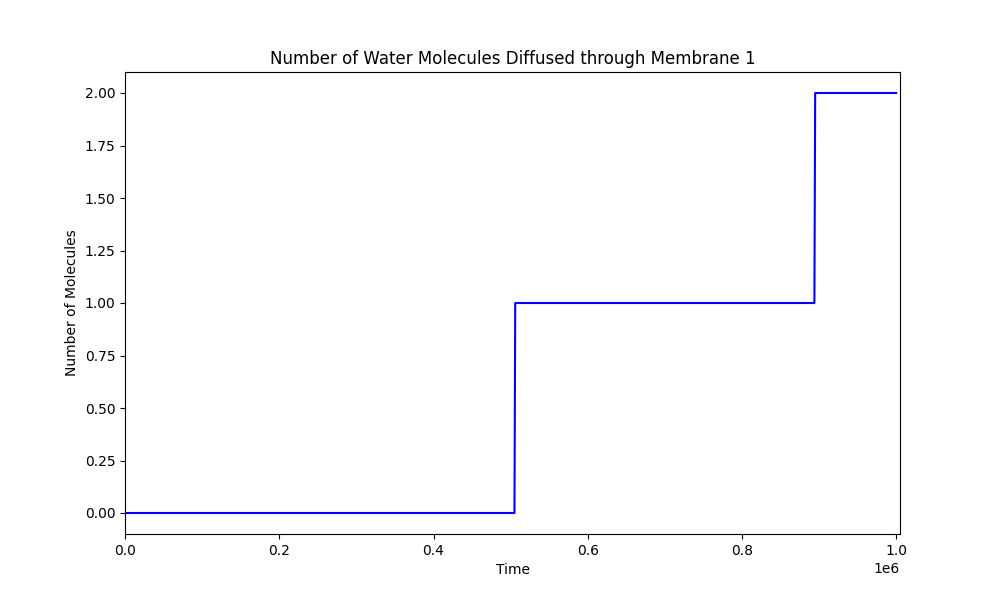
\includegraphics[scale=0.5]{Mem1_1.png} \\
\textbf{154} water molecules crossed through membrane 2. \\
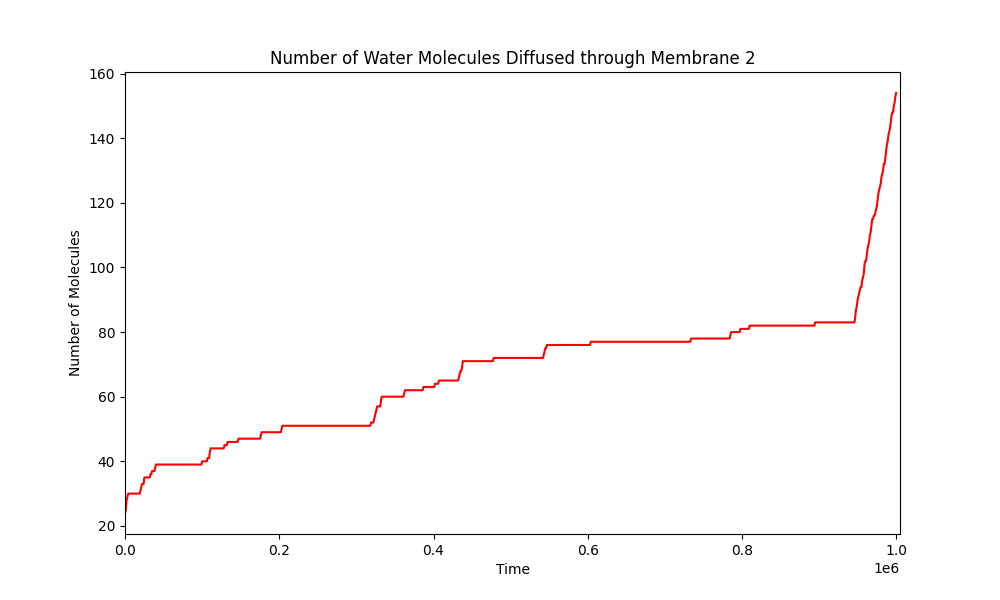
\includegraphics[scale=0.5]{Mem2_1.png} \\ 
\textbf{953} water molecules crossed through membrane 3. \\
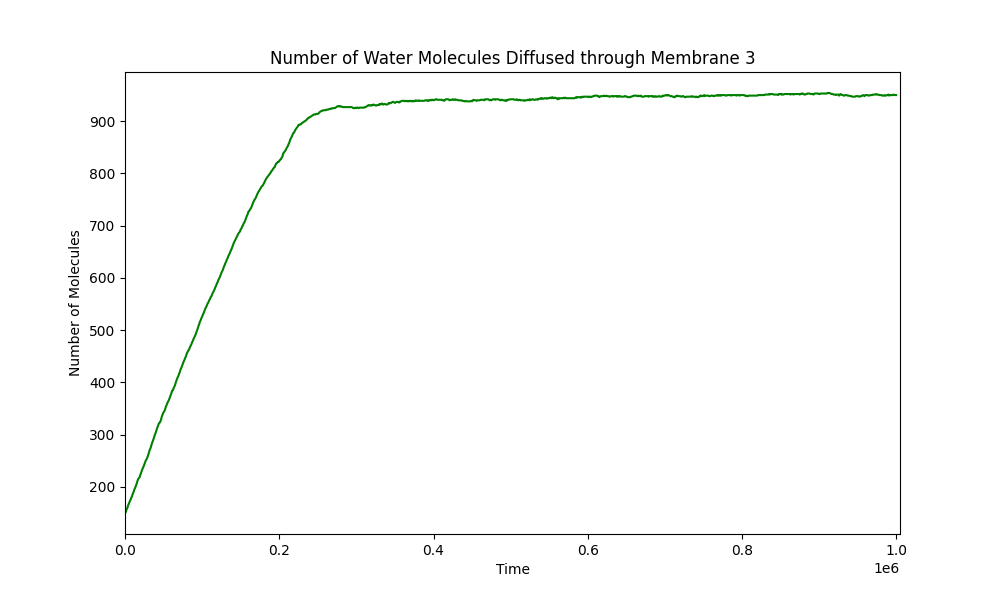
\includegraphics[scale=0.5]{Mem3_1.png} \\ 
In the X axis, the ticks represent the fraction of total time, which is of the order of $10^6$ femtoseconds.

\section{Question 3}

For Membrane 1: \\
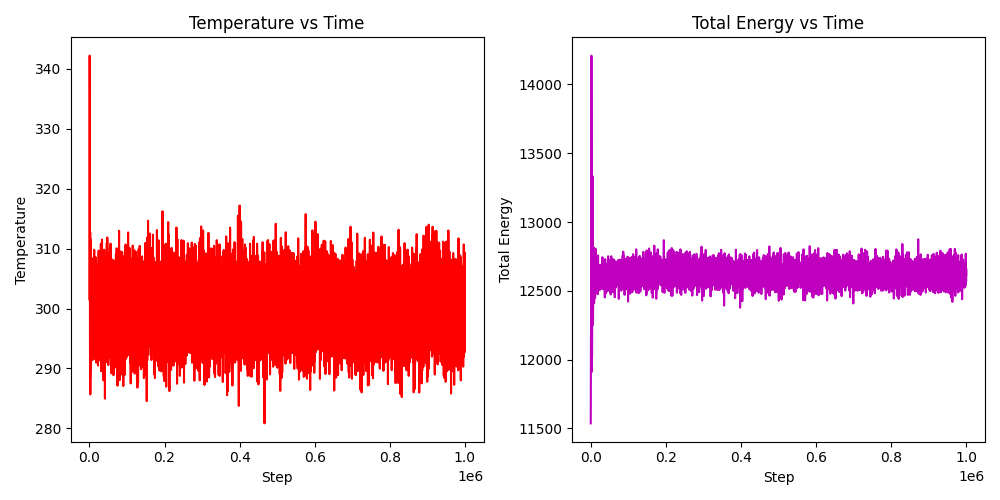
\includegraphics[scale=0.5]{Mem1_2.png} \\

For Membrane 2: \\
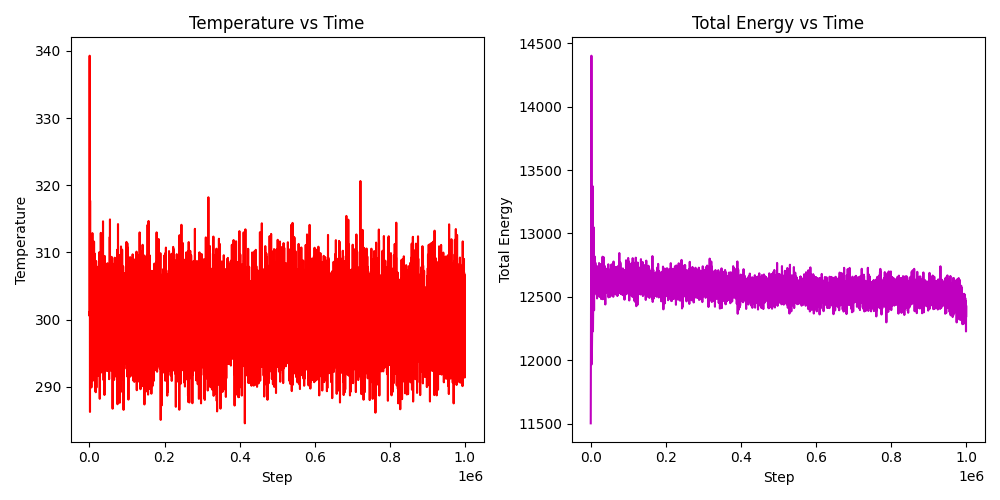
\includegraphics[scale=0.5]{Mem2_2.png} \\

For Membrane 3: \\
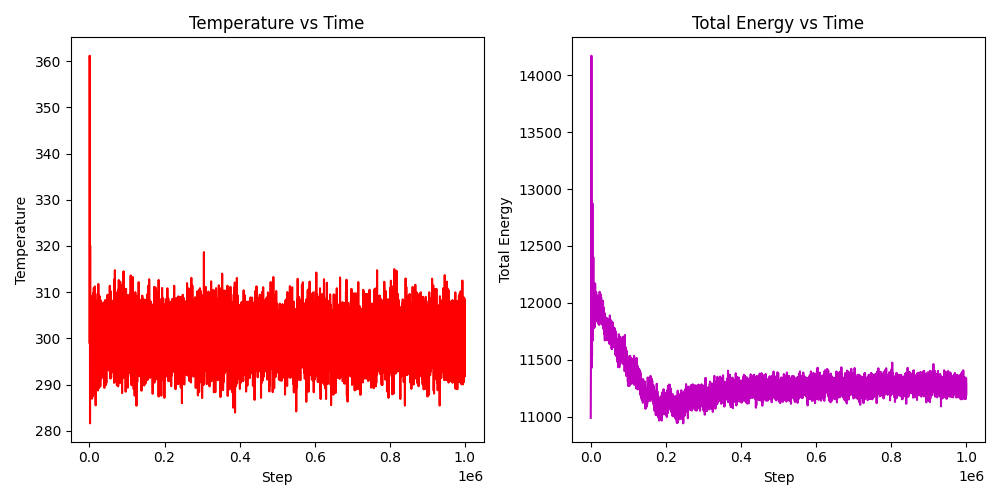
\includegraphics[scale=0.5]{Mem3_2.png} \\ \\
The above plots are for when TDamp is set to 100. Changing the value of Tdamp to 10, and then 1000 for the final nvt runs, yields the following results:\\
For Tdamp = 10: \\
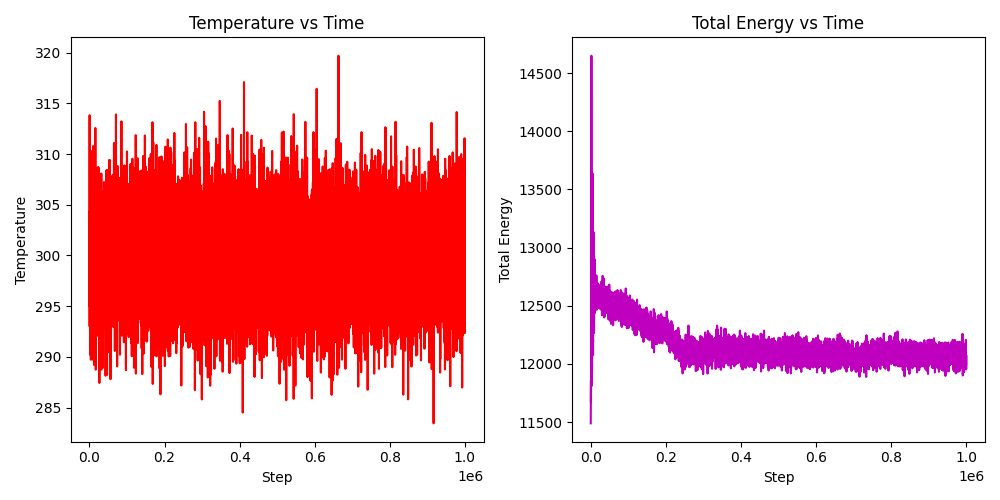
\includegraphics[scale=0.5]{T10.png}\\
For Tdamp = 1000: \\
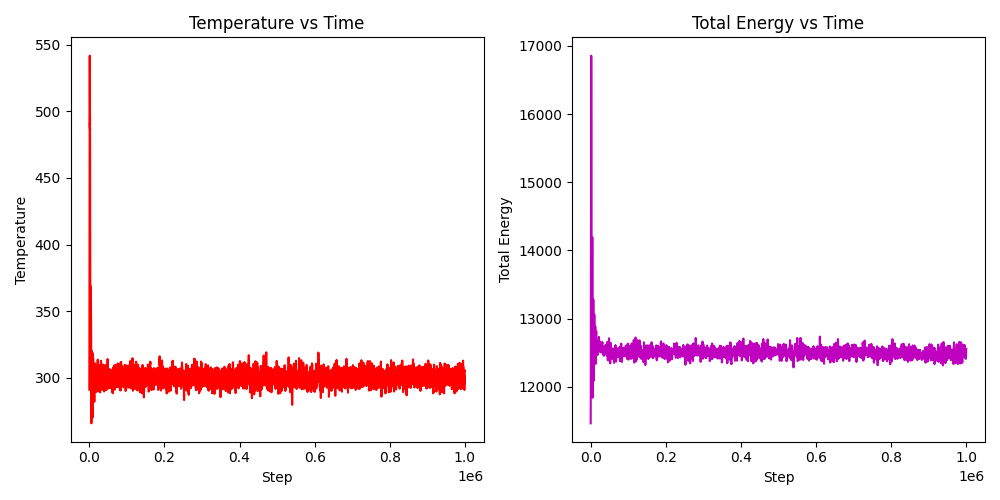
\includegraphics[scale=0.5]{T1000.png}\\
Varying the Tdamp values changes the control parameters, and as can be observed, the less the value of Tdamp, more the system is constrained in its initial stages for system temperatures and total energy.

\section{Question 4}
The plots of the number of molecules of methane crossing the various membranes is given:\\
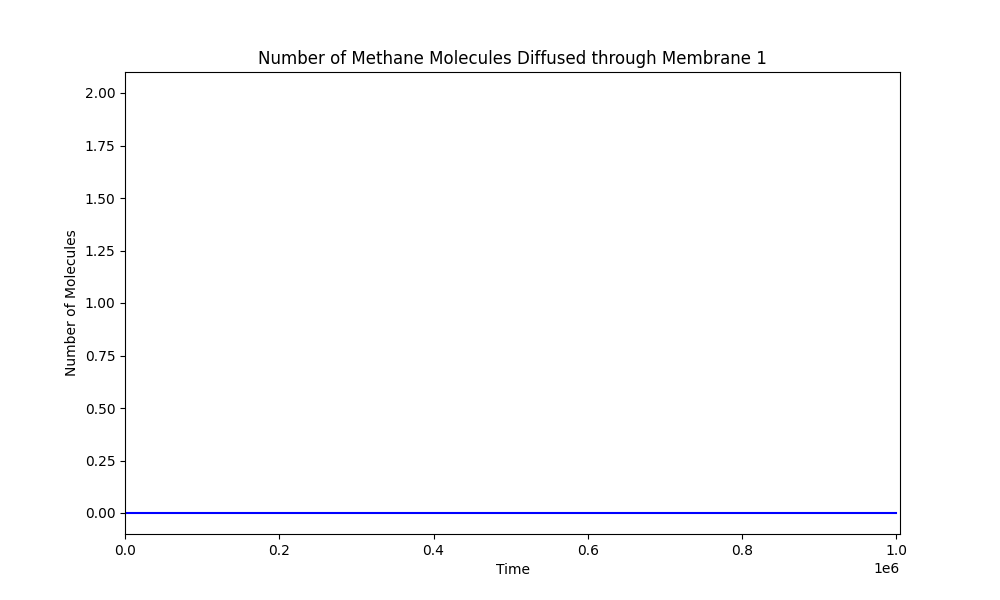
\includegraphics[scale=0.5]{Q4M1.png} \\ 
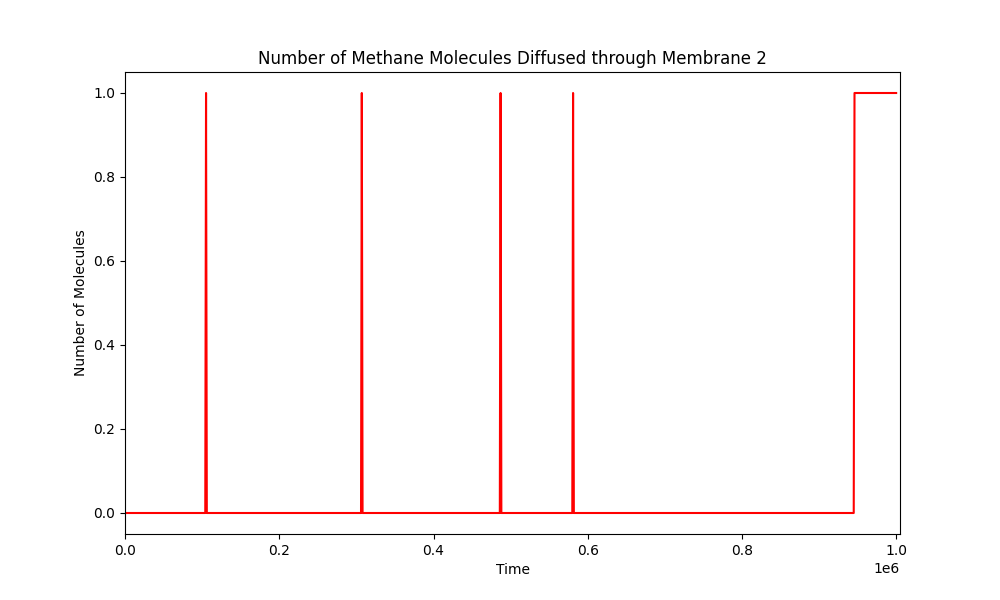
\includegraphics[scale=0.5]{Q4M2.png} \\
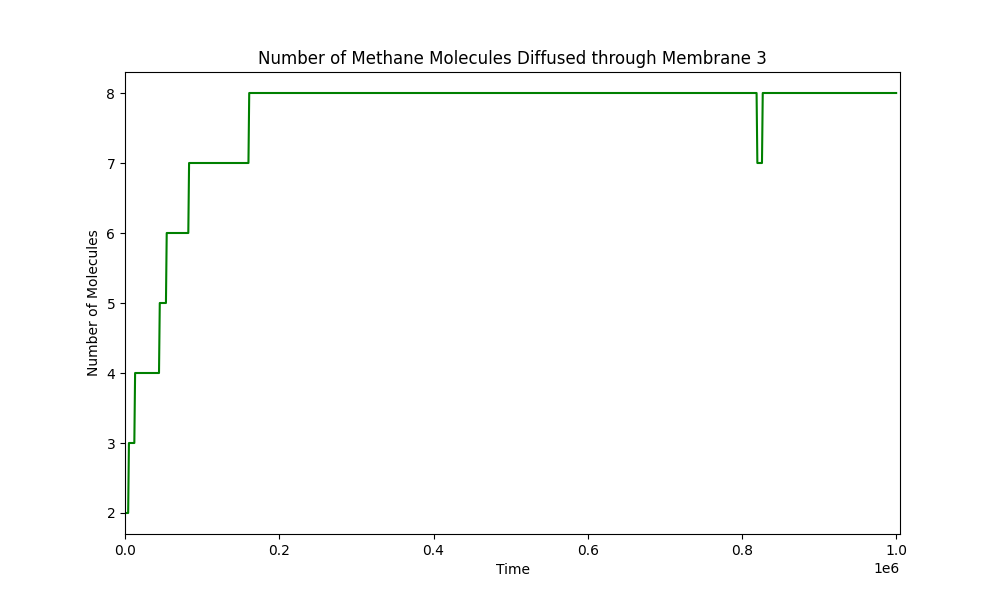
\includegraphics[scale=0.5]{Q4M3.png} \\
Membrane \textbf{2} would be the most effective for filtration, assuming we only want water to be filtered. This is because while the first membrane also stops the diffusion of methane, the number of water molecules passing through it are very low, making it inefficient. In comparison, the second membrane only lets water pass through.

\section{Question 5}
The plots of the number of molecules of Carbon DiOxide crossing the various membranes is given:\\
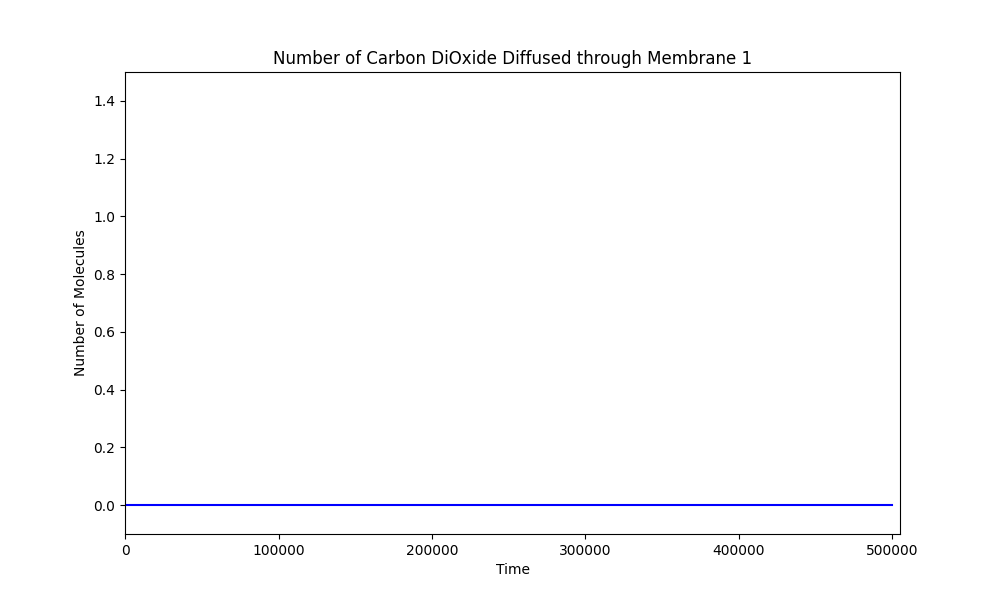
\includegraphics[scale=0.5]{Q5M1.png} \\ 
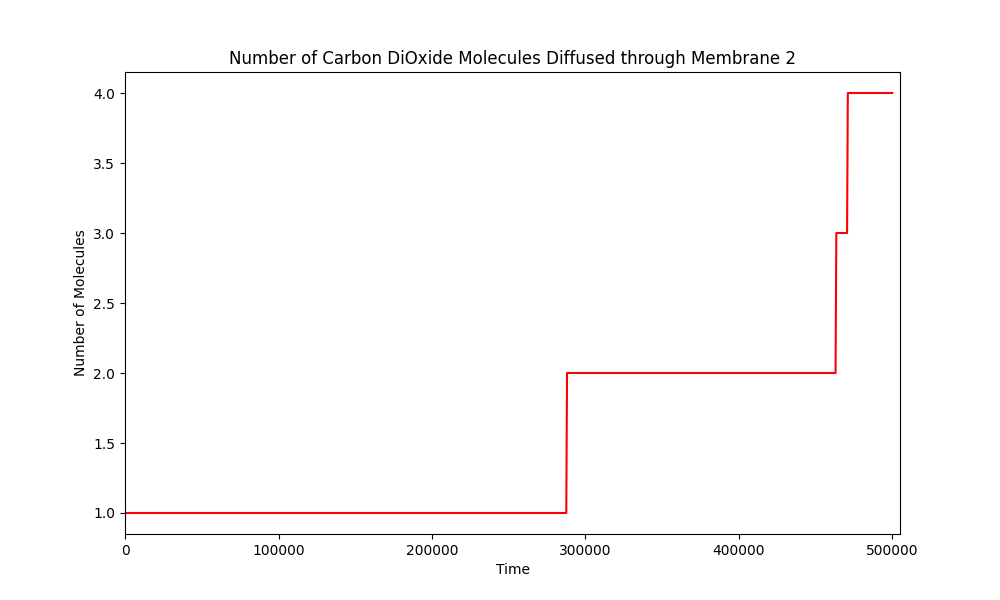
\includegraphics[scale=0.5]{Q5M2.png} \\
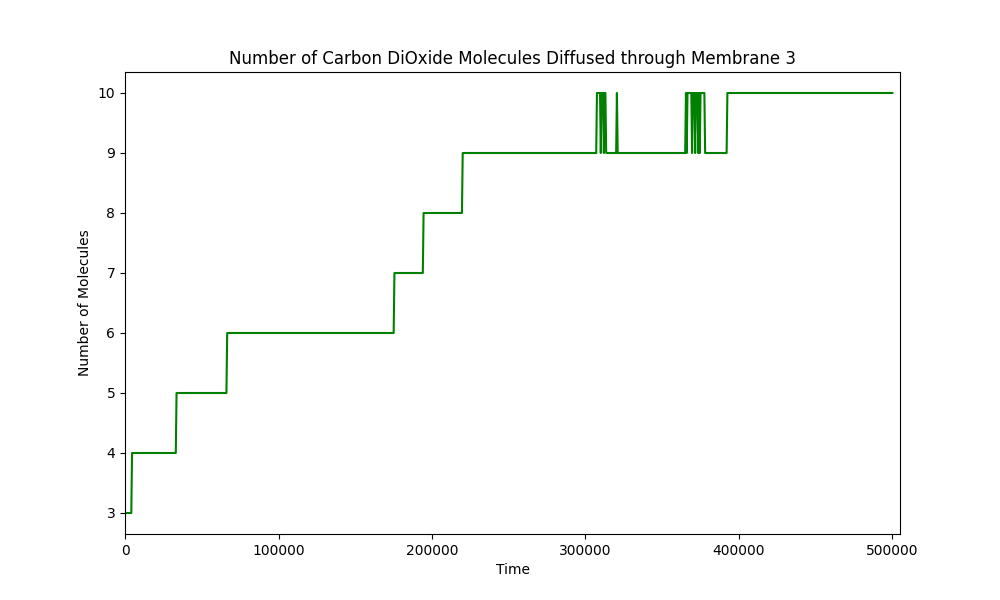
\includegraphics[scale=0.5]{Q5M3.png} \\

Correlating this with the number of water molecules crossing the various membranes: \\
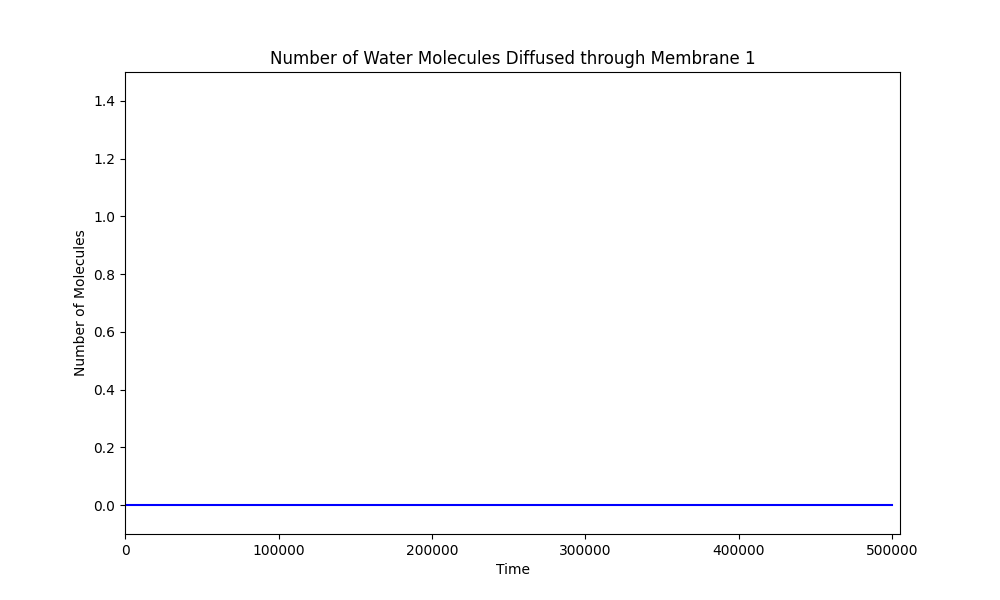
\includegraphics[scale=0.5]{Q5M1_Water.png} \\
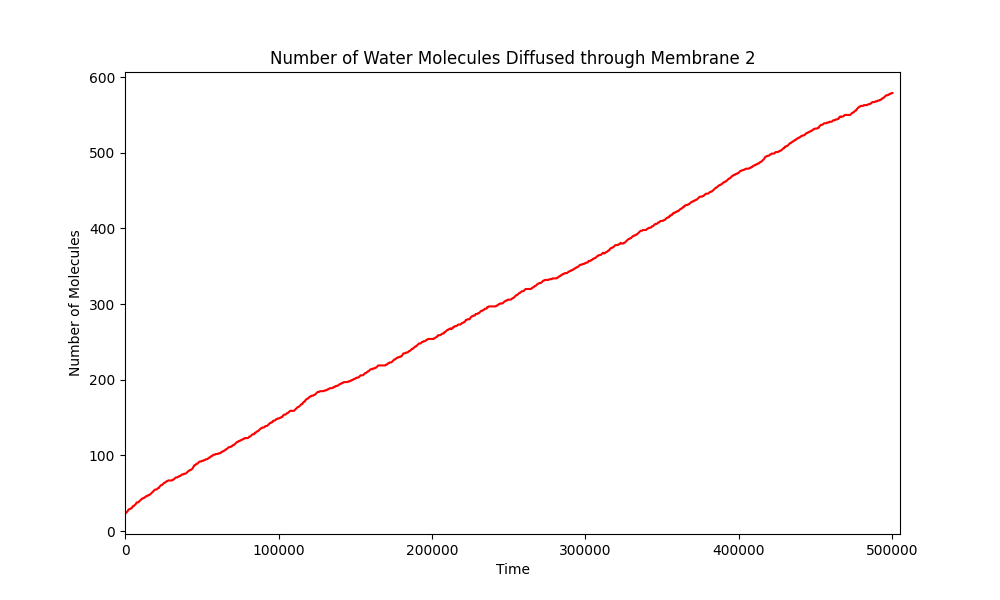
\includegraphics[scale=0.5]{Q5M2_Water.png} \\
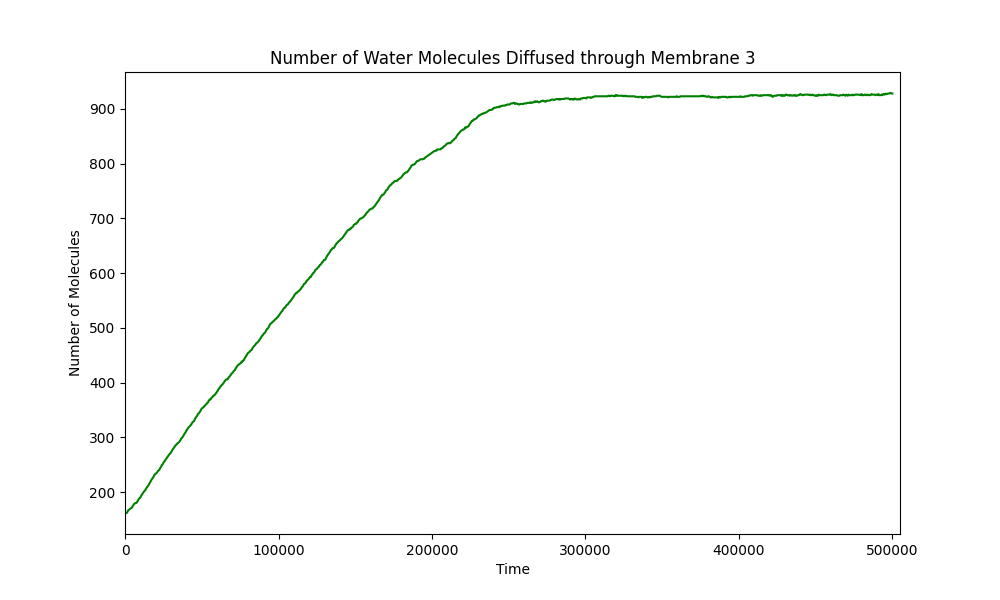
\includegraphics[scale=0.5]{Q5M3_water.png} \\
While Membrane 1 does not allow any $CO_2$ Molecules to pass through, it also doesn't allow any $H_2O$ Molecules to pass through either, making it a very poor permeable membrane. Membrane \textbf{2} allows a very little number of $CO_2$ Molecules to pass through, but a much larger number of $H_2O$ molecules to pass through, which makes it a much better filtration system. \\ \\
\textbf{NOTE:} While the simulations for the $CH_4$ system were done over 1 Million timesteps, the simulations for the $CO_2$ system were done over 500k timesteps. These Timesteps are in femtoseconds, and in plots with fractional X-axes, describe the fraction of $10^6$ femtoseconds.

\end{document}